%%%%%%%%%%%%%%%%%%%%%%%%%%%%%%%%%%%%%%%%%%%%%%%%%%%%%%%%%%%%%%%%%%%%%%%%%%%
%
% Template for a Latex article in English.
%
%%%%%%%%%%%%%%%%%%%%%%%%%%%%%%%%%%%%%%%%%%%%%%%%%%%%%%%%%%%%%%%%%%%%%%%%%%%

\documentclass{article}

% AMS packages:
\usepackage{amsmath, amsthm, amsfonts}
\usepackage{physics}

\usepackage{parskip}
\RequirePackage{graphicx}
\RequirePackage{float}
\RequirePackage{booktabs}
\RequirePackage{enumitem}
\RequirePackage{lipsum}
% si unitx
\RequirePackage{siunitx}
% Theorems
%-----------------------------------------------------------------
\newtheorem{thm}{Theorem}[section]
\newtheorem{cor}[thm]{Corollary}
\newtheorem{lem}[thm]{Lemma}
\newtheorem{prop}[thm]{Proposition}
\theoremstyle{definition}
\newtheorem{defn}[thm]{Definition}
\theoremstyle{remark}
\newtheorem{rem}[thm]{Remark}

\newcommand\hide[1]{}
% Shortcuts.
% One can define new commands to shorten frequently used
% constructions. As an example, this defines the R and Z used
% for the real and integer numbers.
%-----------------------------------------------------------------
\def\R{\mathbb{R}}
\def\Z{\mathbb{Z}}

% Similarly, one can define commands that take arguments. In this
% example we define a command for the absolute value.
% -----------------------------------------------------------------

% Operators
% New operators must defined as such to have them typeset
% correctly. As an example we define the Jacobean:
% -----------------------------------------------------------------
\DeclareMathOperator{\Jac}{Jac}

%-----------------------------------------------------------------
\title{Radioactive Decay}
\author{Scott Fallow, Jeter Hall, Stephen Sekula, Mark Volin*\\
  \small SNOLAB\\
  \small E12345\\
  \small Canada 
}


\begin{document}
\maketitle
\hide{
	\abstract{This is a simple template for an article written in \LaTeX.}
}
\section{Theoretical Background}

\subsection{Radioactive Decay}

\subsubsection{One-Decay Process}

The rate of decay of a single radioactive species is proportional to the amount of atoms in the sample, that is

\begin{equation}
	\dv{t}N=-\lambda N
\end{equation}

where $\lambda$ is the \textit{decay constant}, which is distinct and
characteristic of each isotope. The decay constant is related to the
\textit{half-life} $T_{1/2}$ by

\begin{equation}
	\lambda=\frac{\ln{2}}{T_{1/2}}
\end{equation}

The well known solution too this equation (which can be obtained through a
Laplace transform) is given by

\begin{equation}
	N(t)=\eta e^{-\lambda t}, \qquad \eta:=N(0)
\end{equation}

The \textit{activity} of a radioactive sample refers to the amount of disintegration per unit time

\begin{equation}
	A = \lambda N = -\dv{N}{t}
\end{equation}

given that at any given disintegration the atomic nucleus will emit a particle, the activity also equals the amount of radio-particles emitted per second.

\subsubsection{Multi-Decay Process}

A \textit{decay chain} refers to a series of radioactive decays of different isotopes as a series of transformations, \textit{i.e.} an atom which decays into its child and then decays again into it's grandchild. In this case, the decays are not independent. The number of atoms of a given isotope will depend both on it's own decay rate (by decreasing the number) and the decay rate of it's predecessors (by increasing the number). This scenario is described by Bateman's system of equations:

\begin{equation}
	\dv{F_{i}}{t}=-\lambda_{i}F_{i}(t)+\lambda_{i-1}F_{i-1}(t)
\end{equation}

with $i=1,\; 2,\; 3, \dots, \; k$, $\lambda_{0}\simeq\lambda_{k}\simeq0$ and $k \geq2$. For large enough samples, $F_{i}(t)$ represents the amount of the $i$-th species, which decays into $i+1$ at a rate given by the decay constant $\lambda_{i}$. The reason why $\lambda_{0}\simeq0$ is that we only wish to consider part of the chain, and we are only interested in isotopes with same-scale half-life; take the case of the Uranium Series (Fig. \ref{fig:uranium_series}), Thorium-230 has a half-life of 75.38\unit{\kilo y}, so even when compared to the half-life of Radium-226 (1,682\unit{y}) it's evident that it's decay constant would tend to zero. The same argument goes for $\lambda_{k}$, and specially if that element is considered stable.

\begin{figure}[htb!]
	\centering
	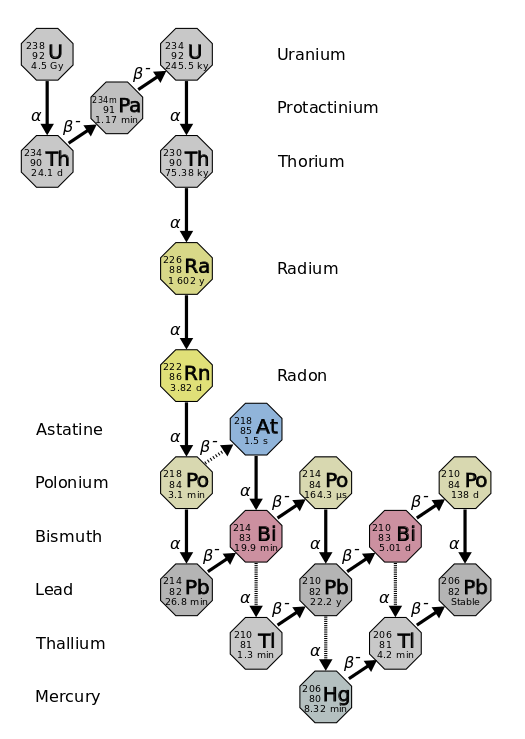
\includegraphics[width=0.5\linewidth]{decay_chain.png}
	\caption{Uranium Series}
	\label{fig:uranium_series}
\end{figure}

It can be easily seen that it the due to th above considerations

\begin{align}
	\dv{t}\sum_{i=1}^{k}F_{i}(t) & =\sum_{i=1}^{k}\dv{F_{i}(t)}{t}=\sum_{i=1}^{k}[-\lambda_{i}F_{i}(t)+\lambda_{i-1}F_{i-1}(t)]            \\
	                             & =\sum_{i=1}^{k}-\lambda_{i}F_{i}(t)+\sum_{i=1}^{k-1}\lambda_{i-1}F_{i-1}(t)=-\lambda_{k}F_{k}(t) \notag \\
	                             & =0\notag
\end{align}

which makes since from a physical point of view, since matter must be conserved.

The system of equations may be written in matrix form as

\begin{equation}
	\begin{pmatrix}
		F_{1}' \\
		F_{2}' \\
		F_{3}' \\
		F_{4}' \\
		F_{5}' \\
	\end{pmatrix}=\begin{pmatrix}
		-\lambda_{1} & 0            & 0            & \cdots & 0            \\
		\lambda_{1}  & -\lambda_{2} & 0            & \cdots & 0            \\
		0            & \lambda_{2}  & -\lambda_{3} & \cdots & 0            \\
		\vdots       & \vdots       & \vdots       & \ddots & \vdots       \\
		0            & 0            & 0            & \cdots & -\lambda_{k} \\
	\end{pmatrix}\begin{pmatrix}
		F_{1} \\
		F_{2} \\
		F_{3} \\
		F_{4} \\
		F_{5} \\
	\end{pmatrix}
\end{equation}

or

\begin{equation}
	\dv{t}F_{i}=L_{ij}F_{j}
	\label{eq:system}
\end{equation}

now, from the one-decay process, we can see the solutions to the system will be given by vectors of the form

\begin{equation}
	F_{i,m}=c_{i,m}e^{-\Lambda_{m}t}
\end{equation}
where the second index refers to the possibility of having more than one solution. Thus, (\ref{eq:system}) can be written as an eigenvalue equation

\begin{equation}
	(L_{ij}-\Lambda_{m}\delta_{ij})F_{j,m}=0
\end{equation}

or taking the non trivial case in which the exponentials are distinct than zero, we can just work with the coefficients

\begin{equation}
	(L_{ij}-\Lambda_{m}\delta_{ij})c_{j,m}=0
\end{equation}

given that $(L_{ij}-\Lambda_{m}\delta_{ij})$ is a triangular matrix, we have

\begin{equation}
	\det(L_{ij}-\Lambda_{m}\delta_{ij})=\prod_{i=1}^{k}(-\lambda_{i}-\Lambda_{m})=0
\end{equation}

Thus, tether are $k$ distinct eigenvalues $\lambda_{m}=-\lambda_{i}$. To each of this eigenvalues there will be an associated eigenvector, each of which corresponds to a independent solution to the system. The general solution to the system will be given by superposing all the independent solutions

\begin{equation}
	\begin{pmatrix}
		F_{1} \\
		F_{2} \\
		F_{3} \\
		F_{4} \\
		F_{5} \\
	\end{pmatrix}=\begin{pmatrix}
		c_{1,1} & c_{1,2} & c_{1,3} & \cdots & c_{1,k} \\
		c_{2,1} & c_{2,2} & c_{2,3} & \cdots & c_{2,k} \\
		c_{3,1} & c_{3,2} & c_{3,3} & \cdots & c_{3,k} \\
		\vdots  & \vdots  & \vdots  & \ddots & \vdots  \\
		c_{5,1} & c_{k,2} & c_{k,3} & \cdots & c_{k,k} \\
	\end{pmatrix}\begin{pmatrix}
		e^{-\Lambda_{1}t} \\
		e^{-\Lambda_{2}t} \\
		e^{-\Lambda_{3}t} \\
		e^{-\Lambda_{4}t} \\
		e^{-\Lambda_{5}t} \\
	\end{pmatrix}
\end{equation}

The coefficients of any given solution will be given by

\begin{equation}
	\begin{pmatrix}
		\lambda_{m}-\lambda_{1} & 0                       & 0                       & \cdots & 0                       \\
		\lambda_{1}             & \lambda_{m}-\lambda_{2} & 0                       & \cdots & 0                       \\
		0                       & \lambda_{2}             & \lambda_{m}-\lambda_{3} & \cdots & 0                       \\
		\vdots                  & \vdots                  & \vdots                  & \ddots & \vdots                  \\
		0                       & 0                       & 0                       & \cdots & \lambda_{m}-\lambda_{k} \\
	\end{pmatrix}\begin{pmatrix}
		c_{1,m} \\
		c_{2,m} \\
		c_{3,m} \\
		c_{4,m} \\
		c_{5,m} \\
	\end{pmatrix}=0
\end{equation}

or, since it was established that $\lambda_{0}\simeq0$,

\begin{equation}
	\lambda_{i-1}c_{i-1,m}=(\lambda_{m}-\lambda_{i})c_{i,m}=0, \qquad i \geq1
\end{equation}

from where we can establish the recurrence relation

\begin{equation}
	c_{i,m}=\left(\frac{\lambda_{i-1}}{\lambda_{i}-\lambda_{m}}\right)c_{i,m}
\end{equation}
% Bibliography
% k
%-----------------------------------------------------------------
\begin{thebibliography}{99}

	\bibitem{Cd94} Author, \emph{Title}, Journal/Editor, (year)

\end{thebibliography}

\end{document}
